\ylDisplay{Maja} % Ülesande nimi
{Jaan Kalda} % Autor
{lahtine} % Voor
{2008} % Aasta
{G 9} % Ülesande nr.
{8} % Raskustase
{
% Teema: Varia
\ifStatement
Juuresolev joonis on tehtud foto põhjal. Pildistamise hetkel asus fotoaparaat \SI{2}{m} kõrgusel veepinnast. Kasutades antud joonist ja joonlauda määrake nii täpselt kui võimalik vees ujuva poi läbimõõt!

\begin{center}
	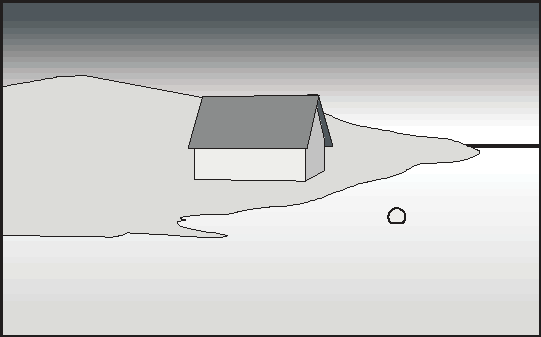
\includegraphics[width=0.9\linewidth]{2008-lahg-09-yl}
\end{center}
\fi


\ifHint
Kõik objektid, mis ületavad fotol horisonti, peavad olema vähemalt sama kõrgel kui fotoaparaat.
\fi


\ifSolution
Joonise põhjal võib oletada, et poi on märksa lähemal horisondist (ca \SI{5}{km}), seega võib Maa kumerust mitte arvestada. Asetame mõtteliselt kahe-meetrise teiba poi kõrvale. Fotoaparaati ja teiba ülemist otsaühendav joon on horisontaalne ja seega läbib horisonti, mis tähendab, et teiba ots puudutab joonisel näha oleva horisondilõigu pikendust. Poi diameetri $d$ leiame mõõtes joonisel pikkused $a$ ja $l$:
\[
d = \SI{2}{m} \cdot \frac al = \SI{45}{cm}.
\]

\begin{center}
	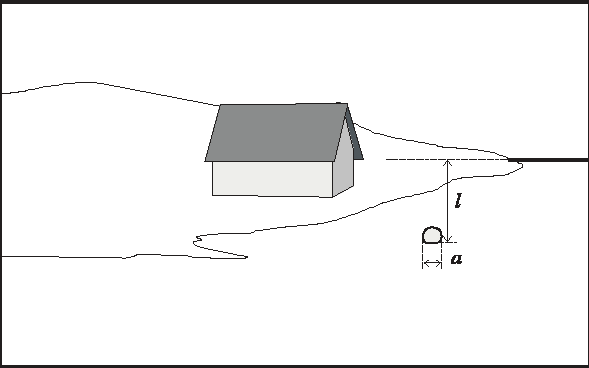
\includegraphics[width=0.9\linewidth]{2008-lahg-09-lah}
\end{center}
\fi
}